\subsection{Preparation for analysis}

We now know some techniques to evaluate raw data, feature by feature and the relationship of features. But a very important step before applying analysis is the preparation, consisting of:
\begin{itemize}
  \item \textbf{Normalization} to make things comparable, 
  \item \textbf{Binning} to make things categorical, and 
  \item \textbf{Sampling} to make data smaller or to change the bias.
\end{itemize}

\subsubsection*{Normalization}
Let's first start with normalization. Typically, when applying normalization\sidenote{Normalization}, values are \textbf{mapped onto a predefined range} while maintaining differences. This predefined range is usually something like $[0, 1]$ or $[-1, 1]$. 

As an example, the following mapping transforms $a_i$ into $a_i'\in[l, h]$ where
\begin{itemize}
  \item $l$ is the lower bound, $h$ the upper one, and
  \item We have a complete set of values $a$ with a defined minimum and maximum given.
\end{itemize}
\begin{align*}
  a_i' = \frac{a_i - \min(a)}{\max(a) - \min(a)} \times (h-l) + l
\end{align*}

Furthermore, we have the \textbf{standard score} using the standard deviation to normalize.
\begin{align*}
  a_i'\sidenote{Standard score} = \frac{a_i - \overline{a}}{sd(a)}\in[-\infty, \infty]
\end{align*}

\subsubsection*{Binning}
Next, we have binning\sidenote{Binning} of values to \textbf{turn continuous} features \textbf{into categorical} ones. Bins are a series of ranges. There are two approaches to determine the bins, both visualized in \ref{fig:2_binning_approaches}.
\begin{itemize}
  \item \textbf{Equal-width binning}\sidenote{Equal-width binning} assumes a fixed width for all bins, where the number of items per bin may vary greatly.
  \item \textbf{Equal-frequency binning}\sidenote{Equal-frequency binning} on the other hand assumes a fixed number of items per bin, but allows a variable width. 
\end{itemize}

\begin{figure}[h]
  \centering
  \begin{subfigure}{0.75\textwidth}
    \centering
    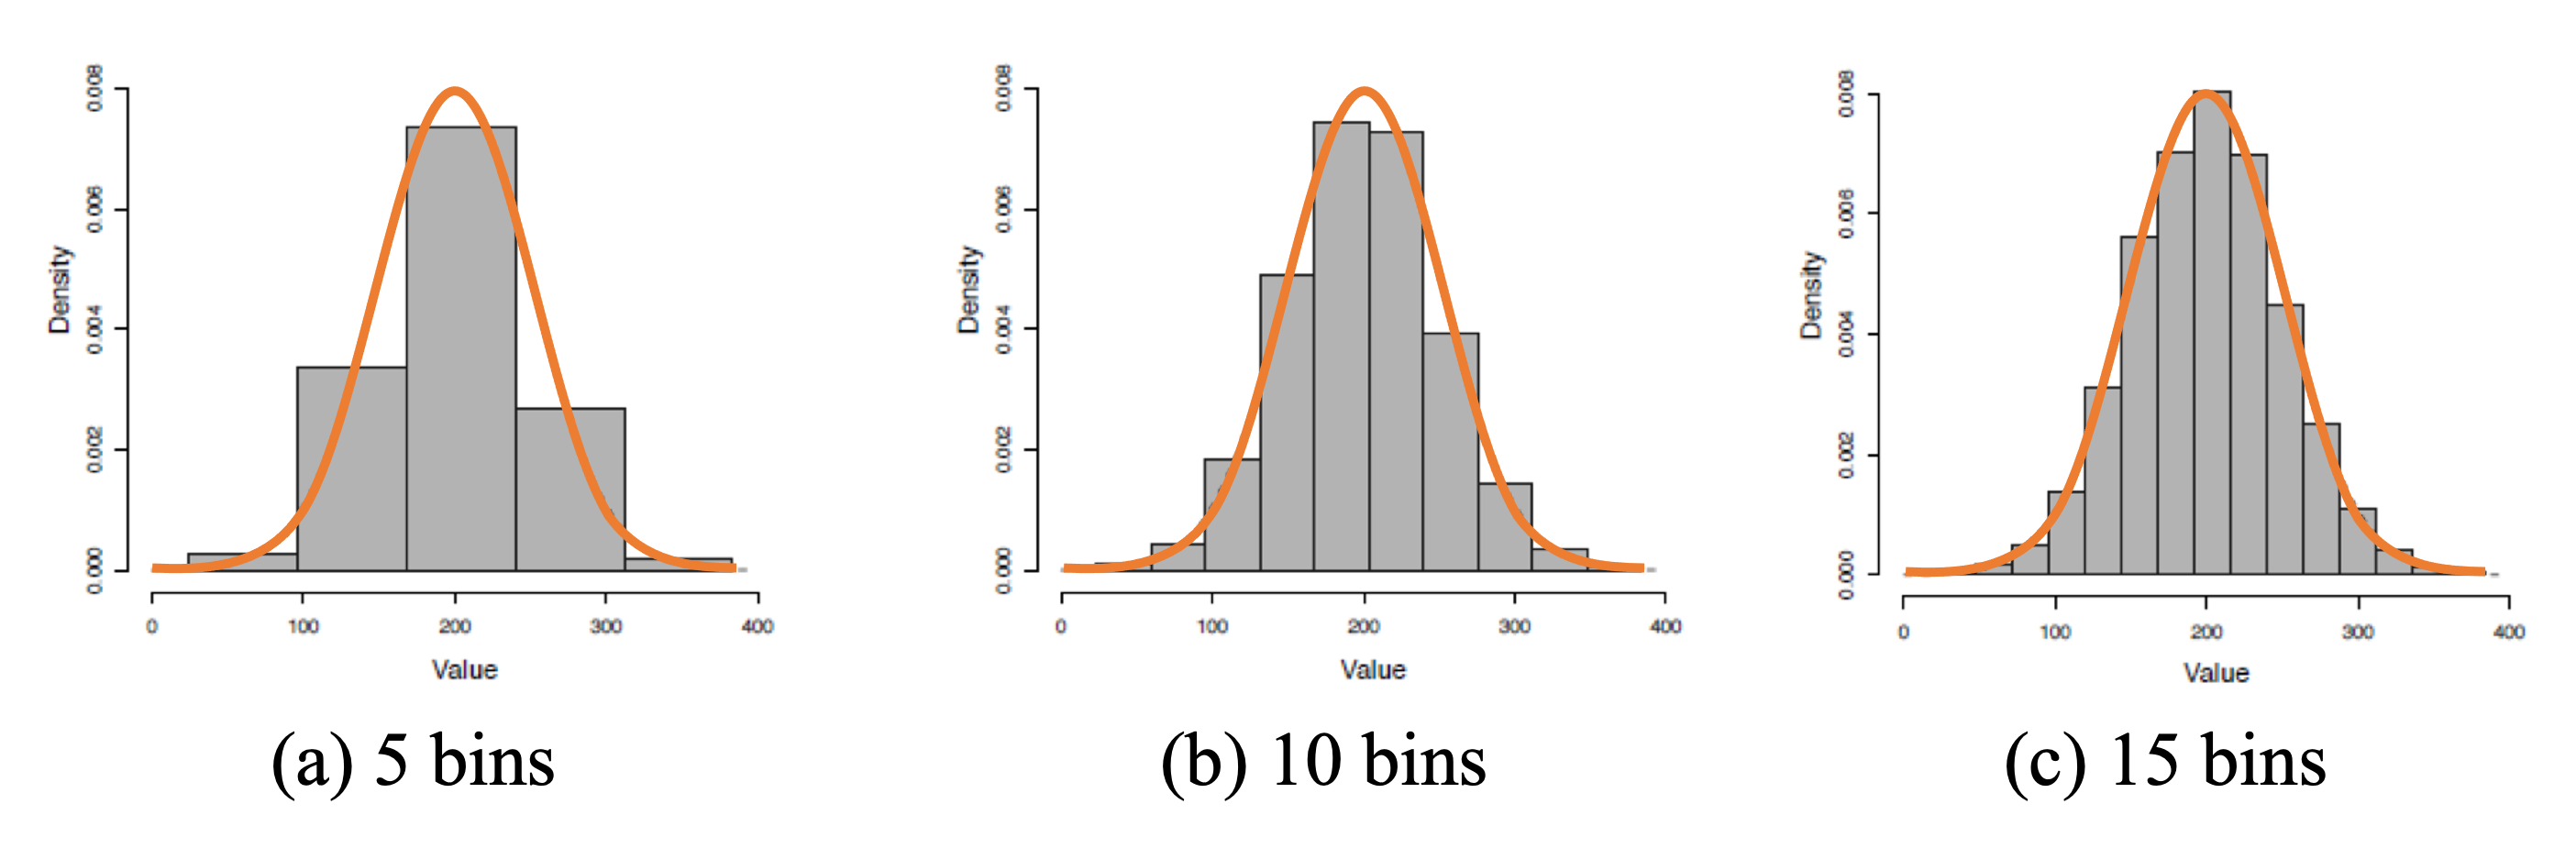
\includegraphics[width=\textwidth]{assets/visualization_and_extraction/prep/bin_equ_width.png}
    \subcaption{Equal-width bins}
  \end{subfigure}

  \vspace*{0.2cm}

  \begin{subfigure}{0.75\textwidth}
    \centering
    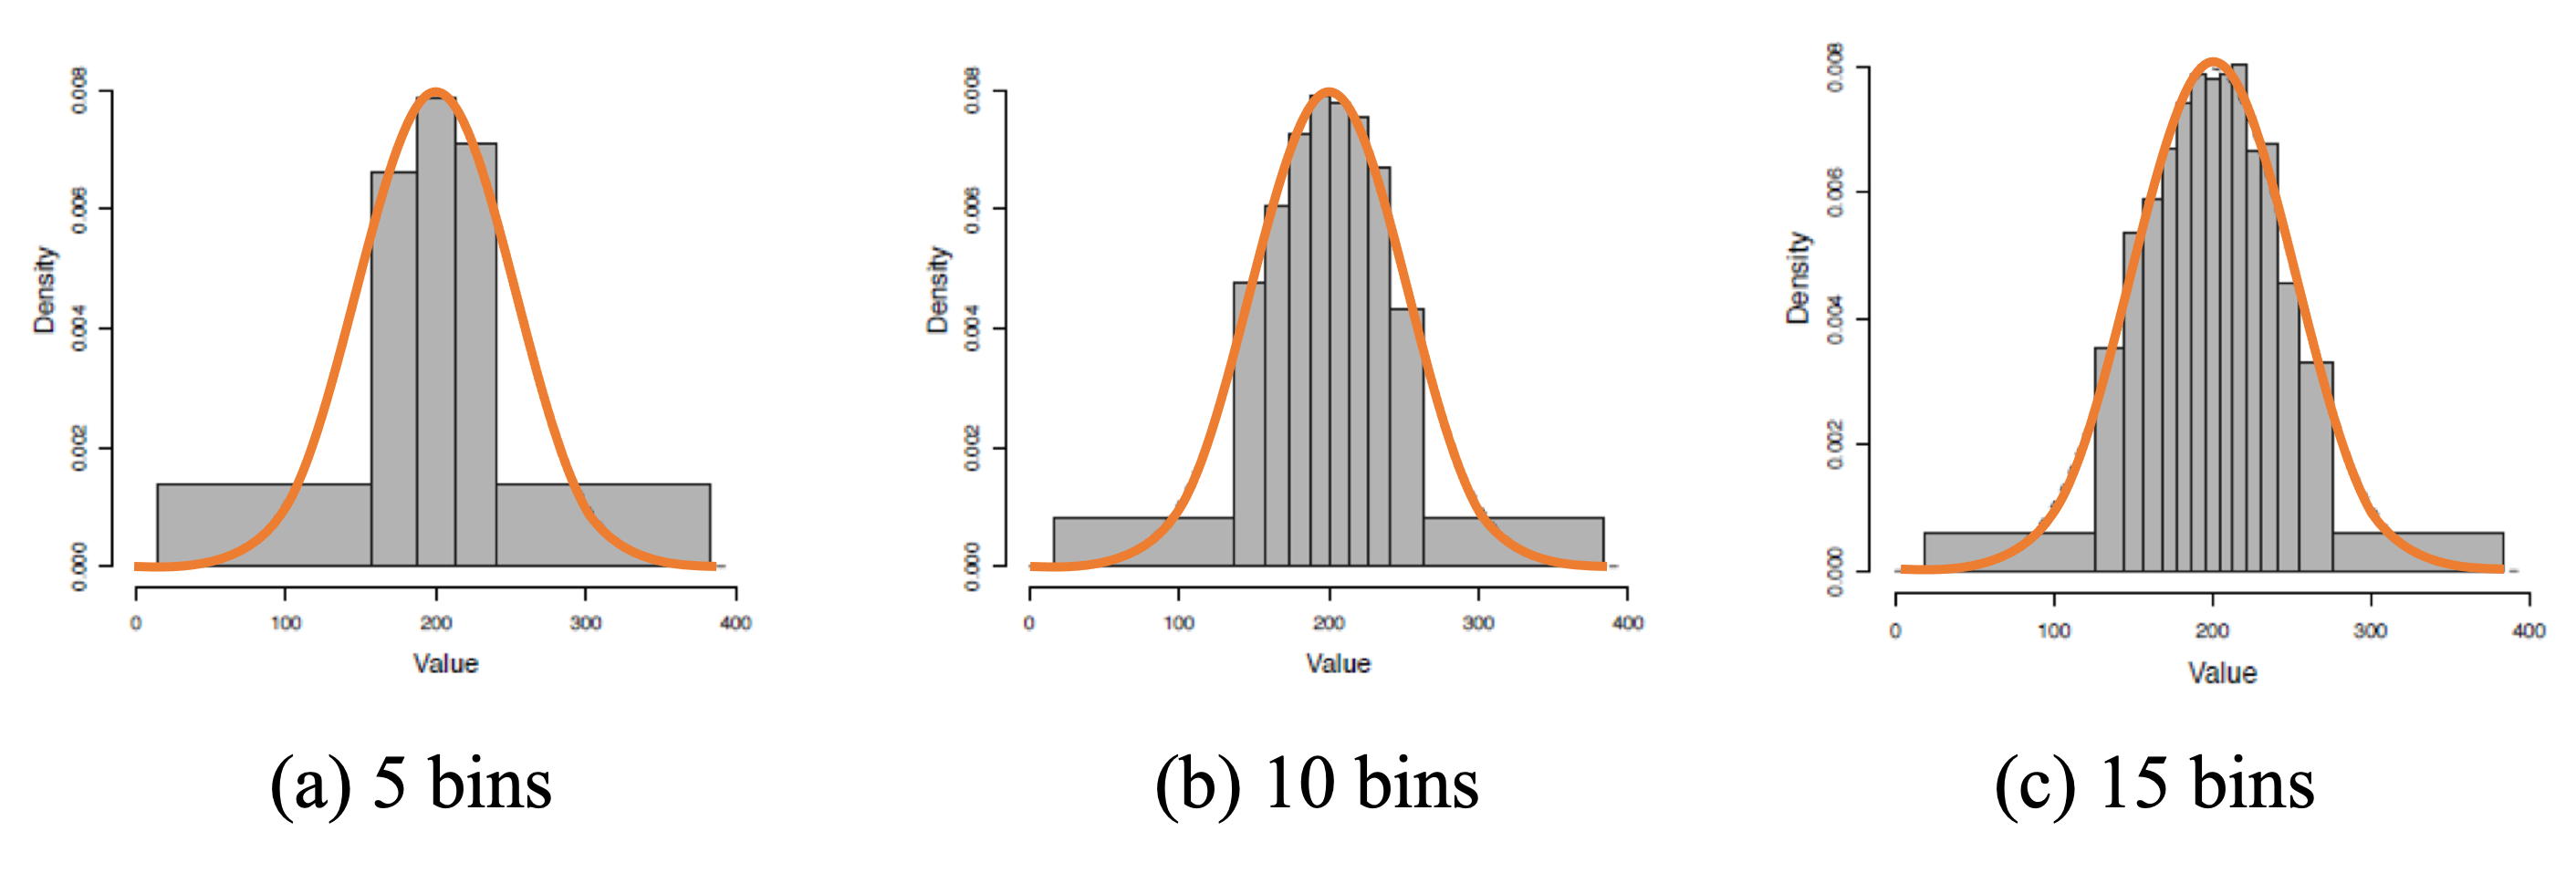
\includegraphics[width=\textwidth]{assets/visualization_and_extraction/prep/bin_equ_frequ.png}
    \subcaption{Equal-frequency bins}
  \end{subfigure}
  \caption{Binning with different number of bins}
  \label{fig:2_binning_approaches}
\end{figure}

The number of items in a bin is reflected by its surface (need to consider both width and height). 

Generally, the number of bins is important as we saw earlier with the problem of over-and under-fitting. 
\begin{itemize}
  \item Underfitting happens when the number of bins is too small, and information gets lost.
  \item Overfitting on the other hand occurs when the number of bins is too large, leading to sparseness with some (nearly) empty bins in areas where the true function considers items to occur very likely.
\end{itemize}

\subsubsection*{Sampling}
Finally, we have the preparation step of sampling\sidenote{Sampling} (which actually ususally comes as the first step). It selects a subset of all available data, and thereby reduces the amount of data. Sampling can remove or introduce a \textbf{sample bias}. 

There are different \textbf{types} of sampling, as depicted in figure \ref{fig:2_sampling_types}.

\begin{figure}[h]
  \centering

  \begin{subfigure}{0.4\textwidth}
    \centering
    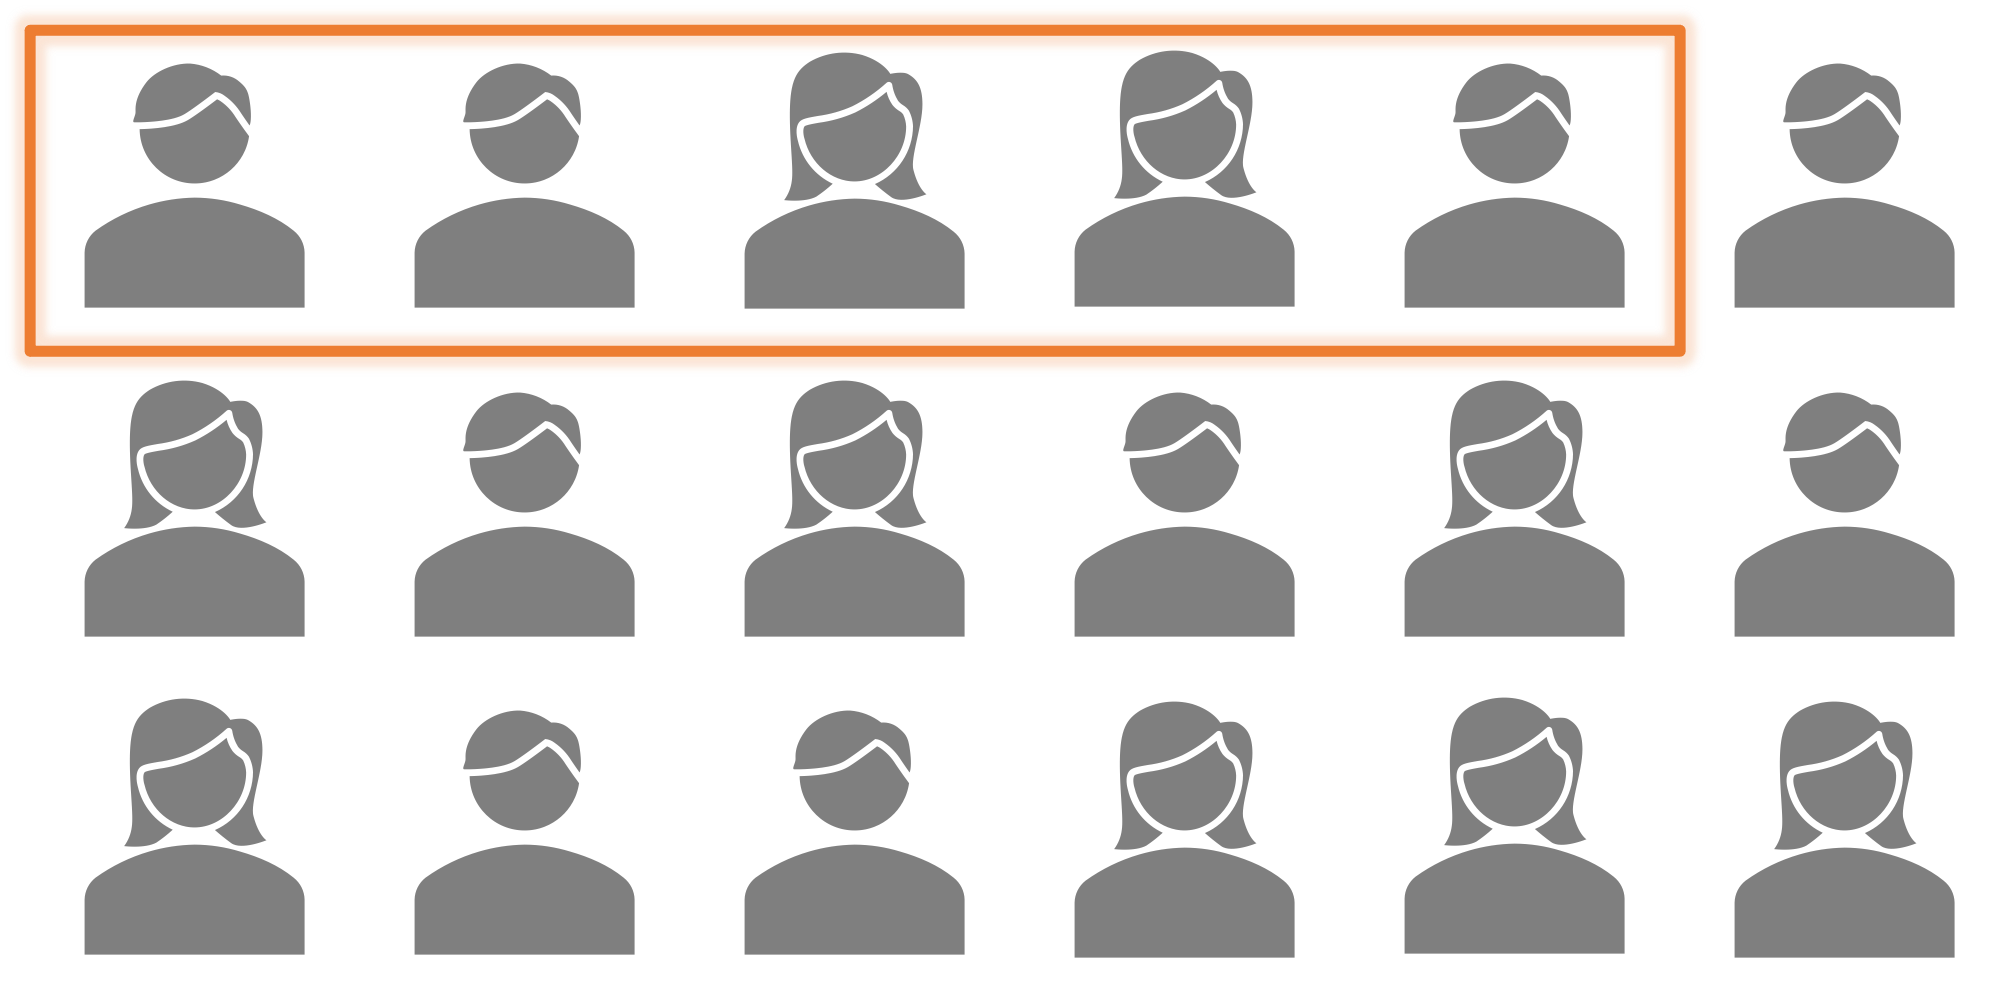
\includegraphics[height=2.3cm]{assets/visualization_and_extraction/prep/sample_top.png}
    \subcaption{Top sampling}
  \end{subfigure}
  \begin{subfigure}{0.4\textwidth}
    \centering
    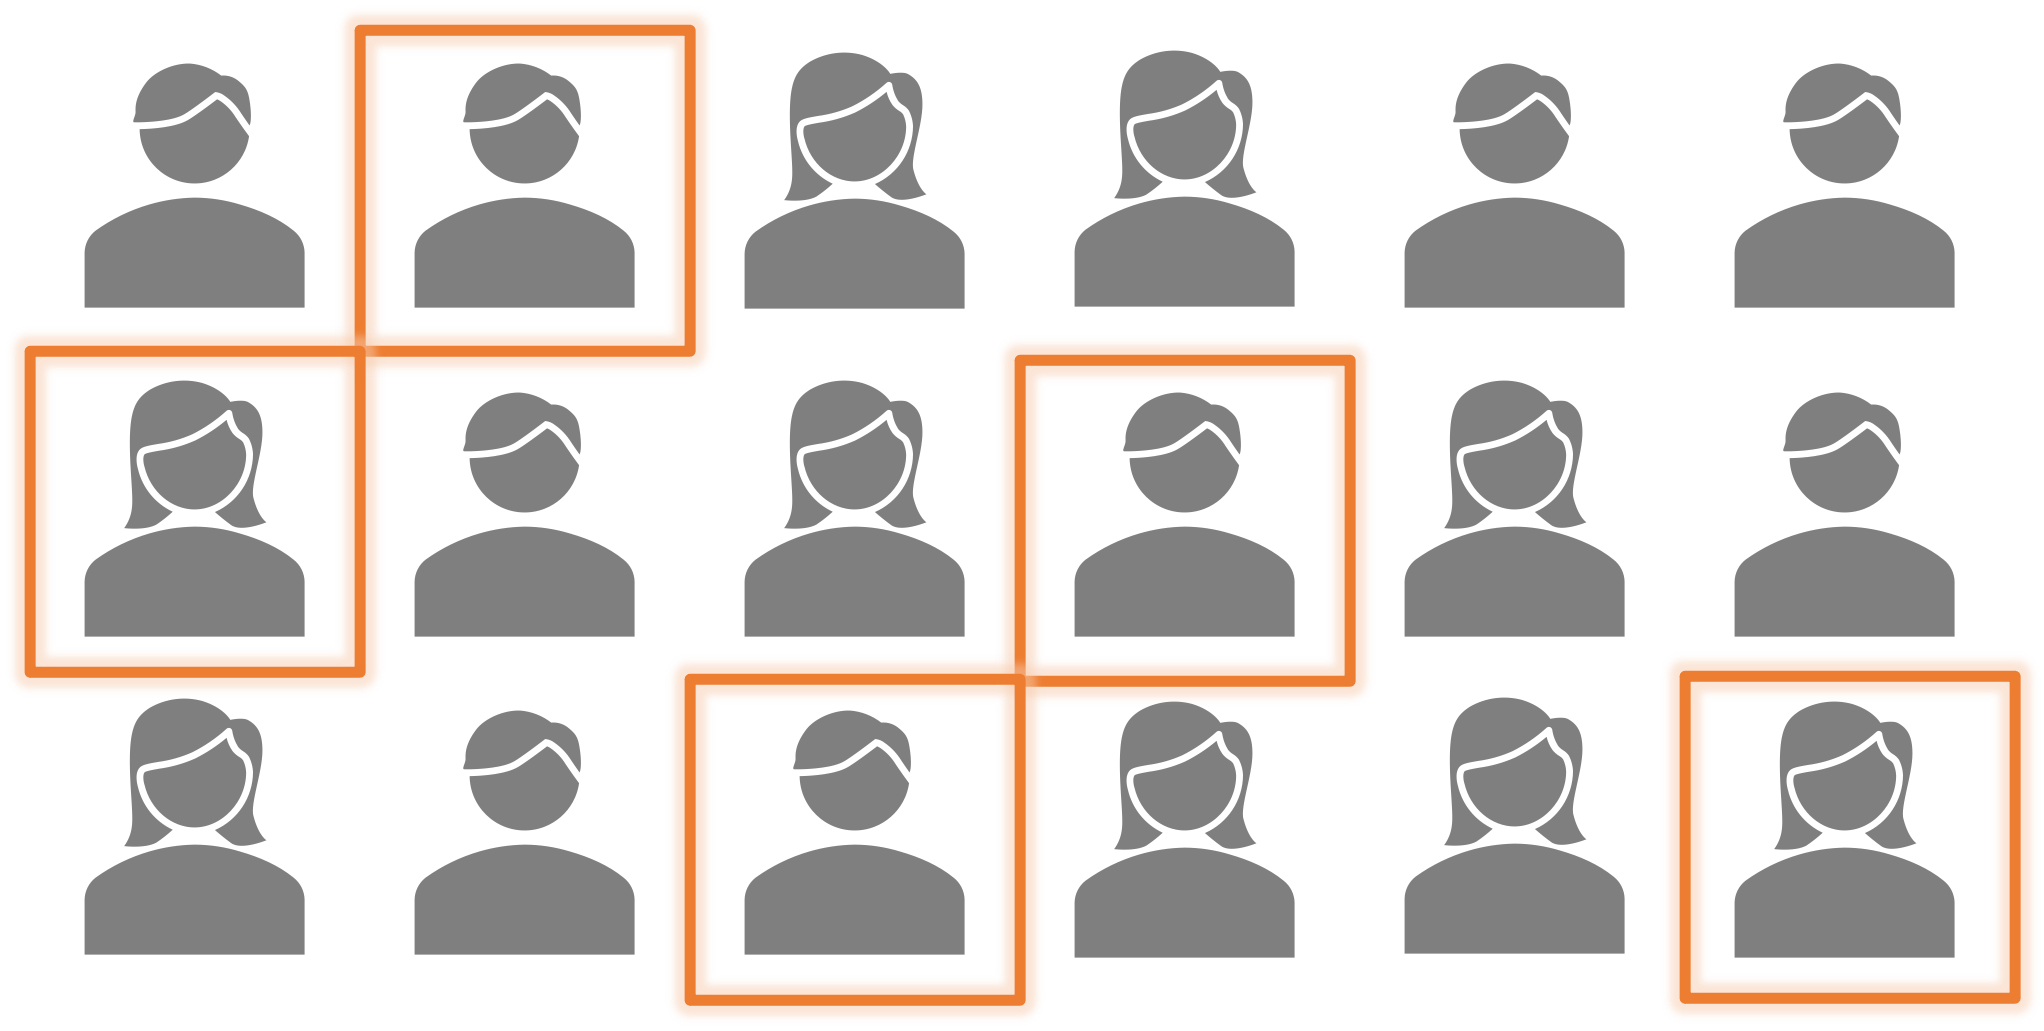
\includegraphics[height=2.3cm]{assets/visualization_and_extraction/prep/sample_random.png}
    \subcaption{Random sampling}
  \end{subfigure}

  \vspace*{0.2cm}
  \begin{subfigure}{0.4\textwidth}
    \centering
    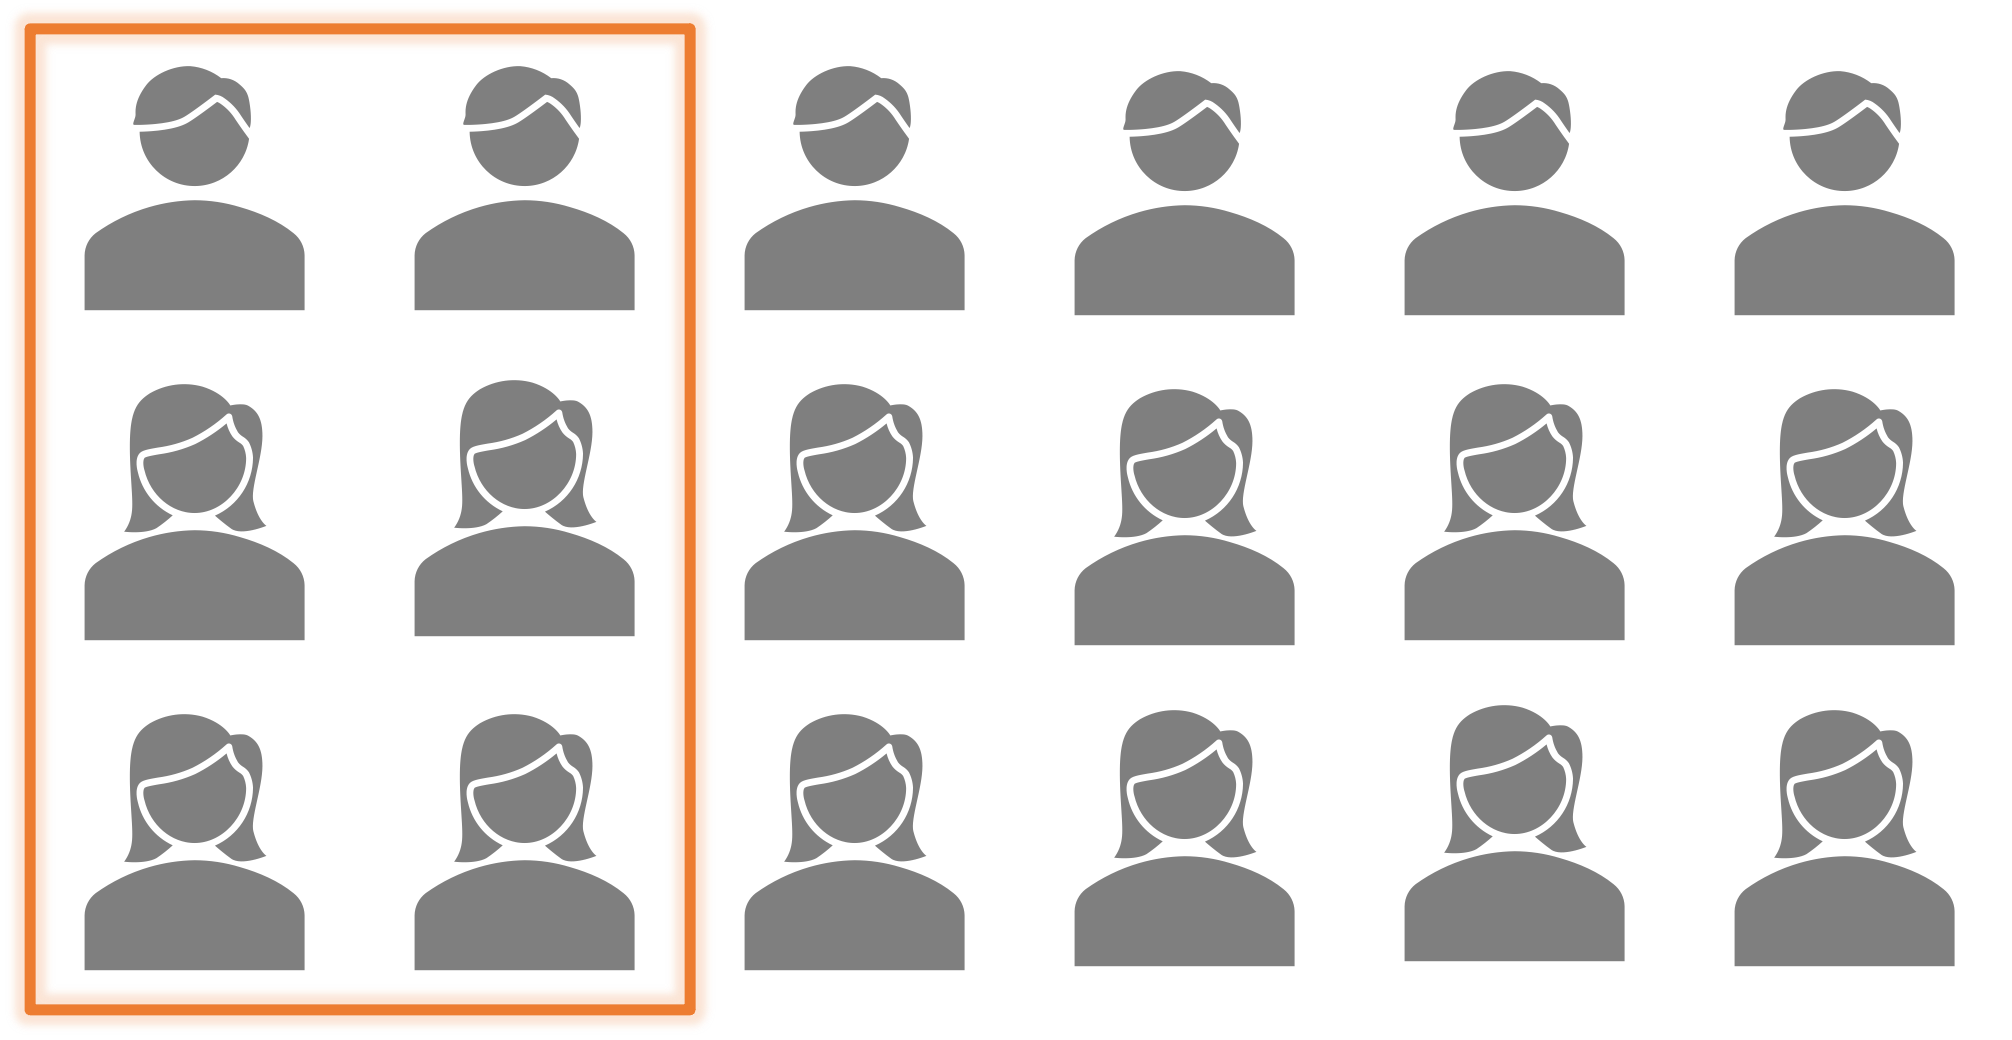
\includegraphics[height=2.3cm]{assets/visualization_and_extraction/prep/sample_stratified.png}
    \subcaption{Stratified sampling}
  \end{subfigure}

  \vspace*{0.2cm}
  \begin{subfigure}{0.4\textwidth}
    \centering
    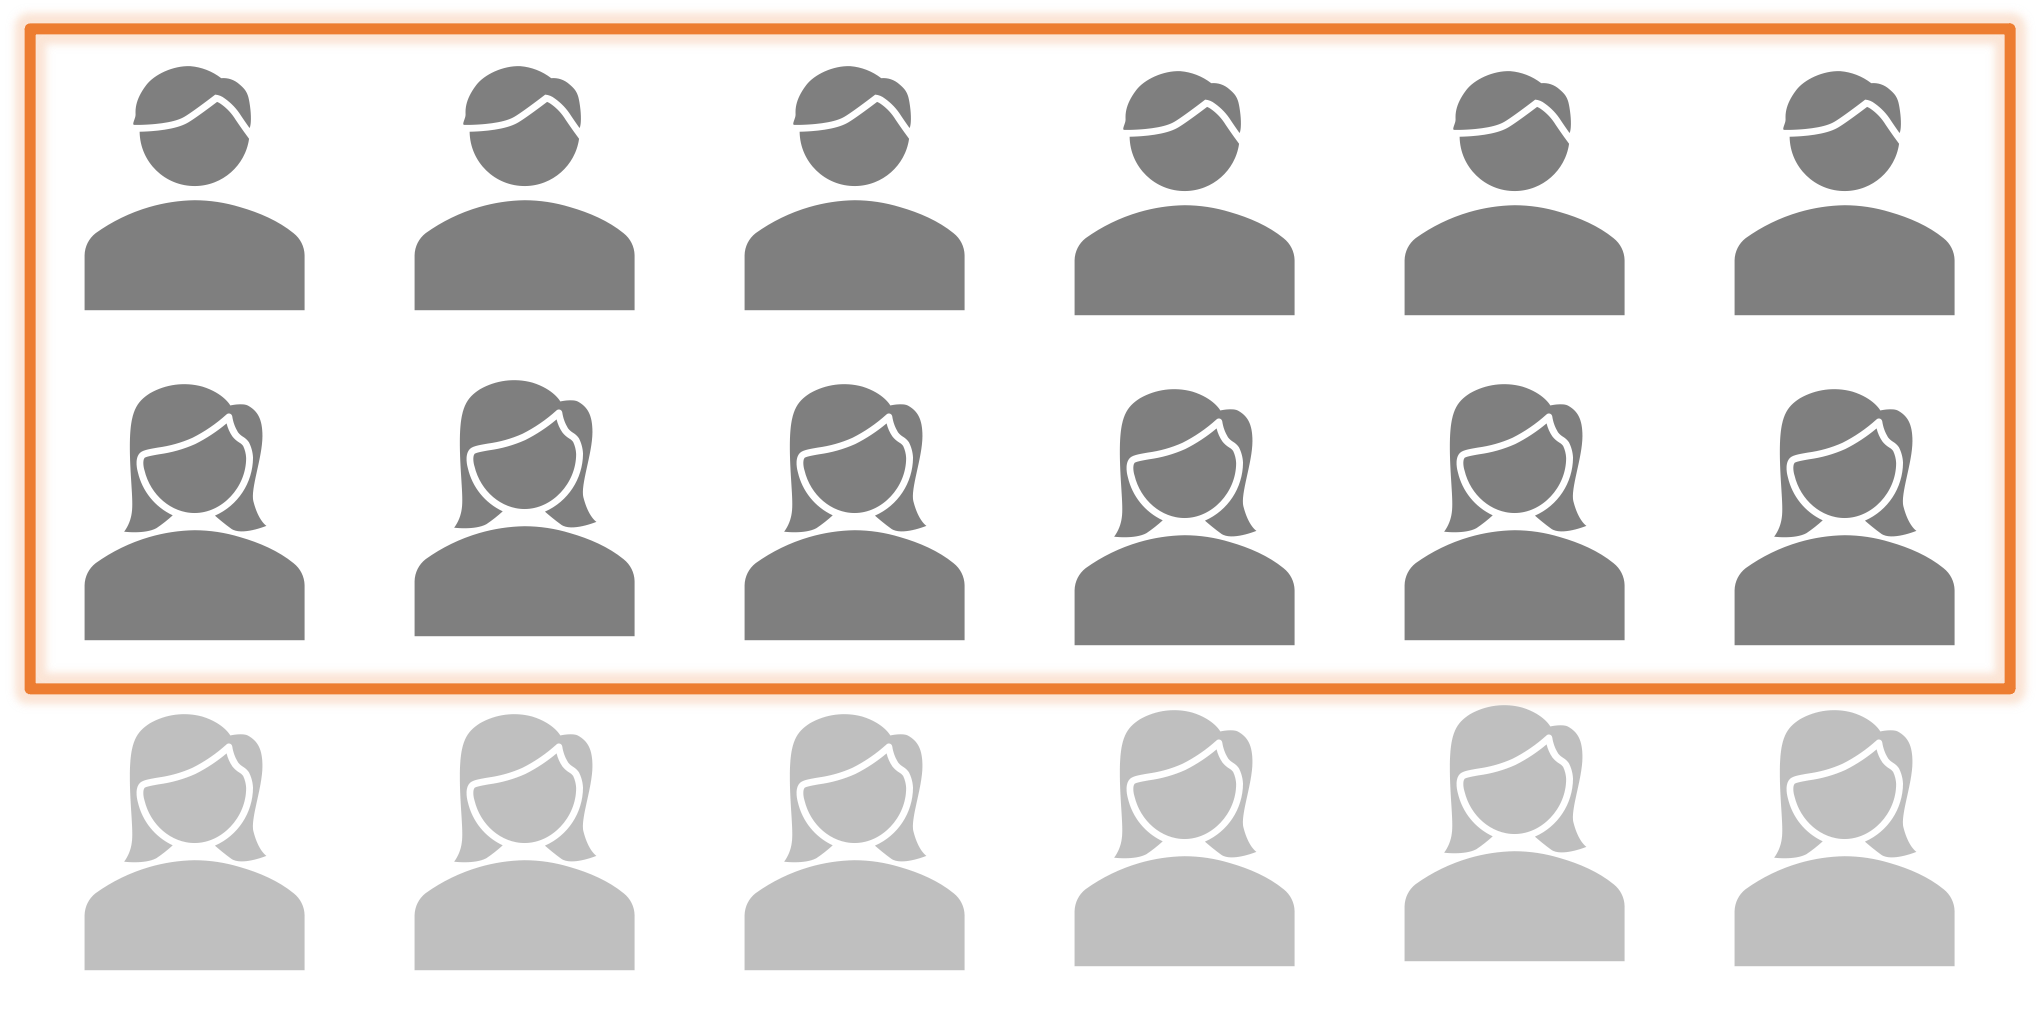
\includegraphics[height=2.3cm]{assets/visualization_and_extraction/prep/sample_under.png}
    \subcaption{Under-sampling}
  \end{subfigure}
  \begin{subfigure}{0.4\textwidth}
    \centering
    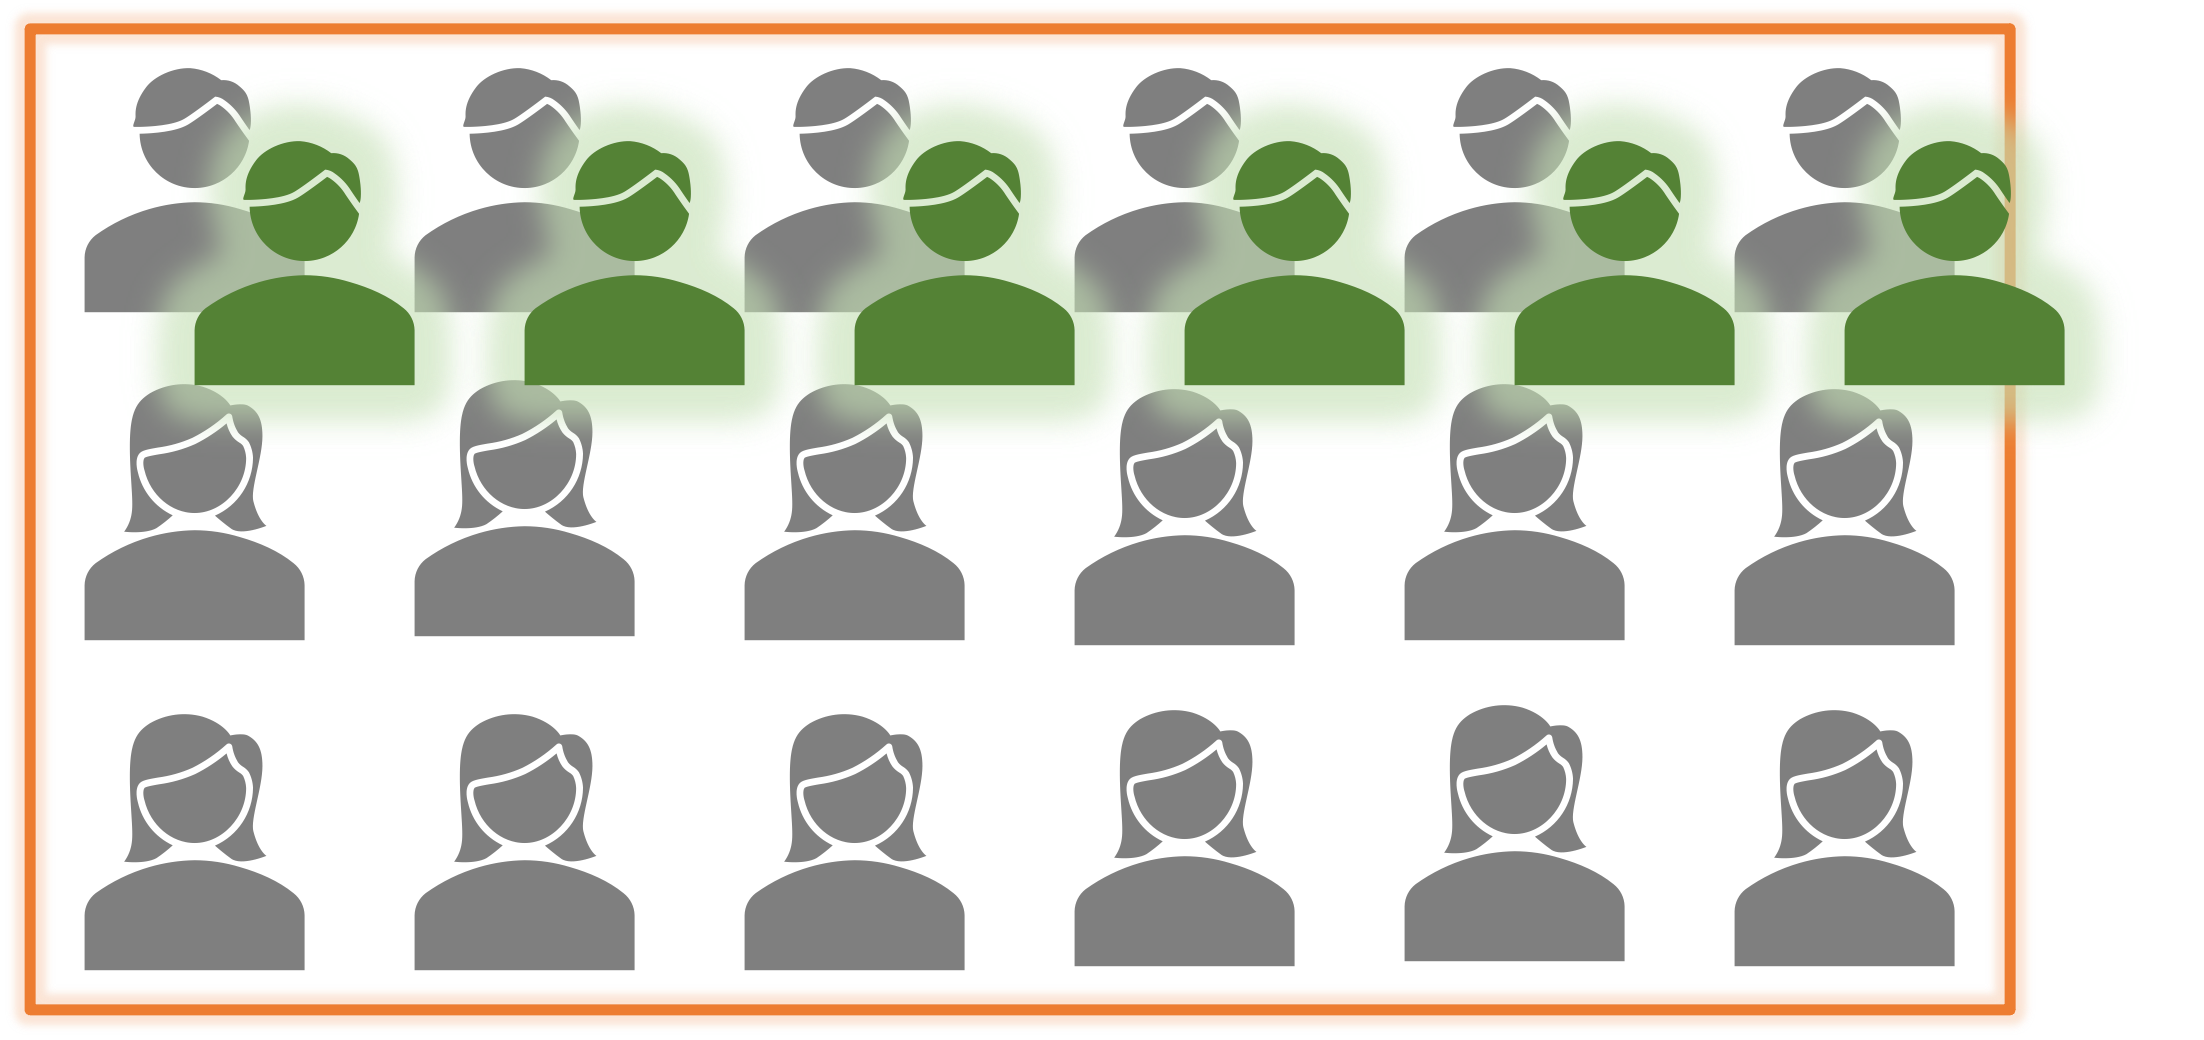
\includegraphics[height=2.3cm]{assets/visualization_and_extraction/prep/sample_over.png}
    \subcaption{Over-sampling \textcolor{gray}{\footnotesize  (The green instances are replicas)}}
  \end{subfigure}
  \caption{Types of sampling}
  \label{fig:2_sampling_types}
\end{figure}

\begin{itemize}
  \item \textbf{Top} sampling takes the first $n$ instances
  \item \textbf{Random} sampling
  \item \textbf{Stratified} sampling where the relative frequencies are ensured to be maintained \textcolor{gray}{\footnotesize (e.g. by taking the same percentage from every group)}
  \item \textbf{Under}-sampling, where balance between groups is ensured by leaving out instances of over-represented groups.
  \item \textbf{Over}-sampling, where balance between groups is ensured by duplicating under-represented groups.
\end{itemize}

